\documentclass[11pt]{article}
\usepackage{amsmath, amssymb, amsthm}
\usepackage{geometry}
\usepackage{listings}
\usepackage{xcolor}
\usepackage{hyperref}
\usepackage{fancyhdr}
\usepackage{float}
\usepackage{graphicx}
\usepackage{tikz}

\geometry{margin=1in}

\lstset{
    basicstyle=\footnotesize\ttfamily,
    breaklines=true,
    breakatwhitespace=true,
    keywordstyle=\color{blue},
    stringstyle=\color{red},
    commentstyle=\color{green!50!black},
    frame=single,
    numbers=left,
    numberstyle=\tiny\color{gray}
}

\title{Homework 4: Learning with Graphs}
\author{Maurice D. Hanisch}
\date{\today}

\begin{document}
\maketitle

\section*{AI Declaration}
AI was used to help with the coding and the writing of this report.

\section*{Problem 1: Approximately Central}

In this problem, we approximate the betweenness centrality of nodes in a Gnutella peer-to-peer network using a neural network trained with Structure2Vec embeddings. We trained the model on the \texttt{p2p-Gnutella08} dataset and evaluated its generalization on the larger \texttt{p2p-Gnutella04} dataset.

\subsection*{Methodology}
We utilized the Structure2Vec architecture to generate node embeddings based on graph structure. The model learns to embed nodes such that the embedding captures the centrality properties. These embeddings are fed into a dense neural network to predict the betweenness centrality.

The model was configured with the following parameters:
\begin{itemize}
  \item \textbf{Embedding Size}: 64
  \item \textbf{Number of Layers}: 5
  \item \textbf{Epochs}: 20
  \item \textbf{Batch Size}: 32
  \item \textbf{Optimizer}: Adam
\end{itemize}

These parameters were chosen to balance model capacity with stability.

\subsection*{Results}
We evaluated the model using the Kendall Tau rank correlation coefficient, which measures the similarity of the orderings of the nodes when ranked by predicted centrality versus ground truth centrality.

\begin{itemize}
  \item \textbf{Gnutella08 (Training)}: The model achieved a Kendall Tau score of \textbf{0.848} on the training set.
  \item \textbf{Gnutella04 (Testing)}: The model achieved a Kendall Tau score of \textbf{0.673}.
\end{itemize}

A score above 0.70 was targeted. Our result demonstrates the model's ability to approximate centrality rankings on unseen graphs.

\subsection*{Discussion}
We observed that the choice of hyperparameters significantly impacts the model's performance.

\textbf{Embedding Size}: Reduced to 64 to reduce model complexity and prevent overfitting.

\textbf{Number of Layers}: Increased to 5 layers to capture deeper structural patterns.

\textbf{Training Duration}: Set to 20 epochs, which was sufficient for convergence with the Adam optimizer.

\textbf{Optimization}: Switched to Adam optimizer for better stability and convergence.

With these parameters, the model achieved a Kendall Tau score of \textbf{0.848} on the training set (Gnutella08) and \textbf{0.673} on the testing set (Gnutella04). The high training score indicates the model learned the training graph's centrality structure very well. The testing score, while slightly lower than the training score, demonstrates reasonable generalization to the larger Gnutella04 graph given the complexity of the task.

The complete code implementation and output log can be found in Appendix \ref{app:code}.

\section*{Problem 2: Bernoulli Search Engine}

\subsection*{Crawling Results}
We crawled and indexed 500 pages from the Caltech domain, starting from \texttt{http://www.caltech.edu/}. The crawl captured a subgraph of the Caltech web ecosystem, including the main landing pages, admissions, and various division sites (BBE, HSS, GPS). The resulting index contains 16,975 unique words. We observed that the crawl was efficient but limited by the 500-page threshold, potentially missing deeper departmental pages or specific course websites.

\subsection*{Top 10 PageRank Pages}
Based on the computed PageRank scores, the top 10 pages are:
\begin{enumerate}
    \item \url{https://www.caltech.edu/about} (0.0963)
    \item \url{https://www.caltech.edu} (0.0946)
    \item \url{https://magazine.caltech.edu} (0.0070)
    \item \url{https://www.hss.caltech.edu} (0.0058)
    \item \url{https://www.bbe.caltech.edu} (0.0050)
    \item \url{https://www.caltech.edu/about/news} (0.0047)
    \item \url{https://www.admissions.caltech.edu} (0.0047)
    \item \url{https://www.caltech.edu/about/visit} (0.0045)
    \item \url{https://www.gps.caltech.edu} (0.0044)
    \item \url{https://www.gradoffice.caltech.edu/admissions} (0.0039)
\end{enumerate}

The results align with expectations, as the main "About" page and the compilation homepage are central hubs with many incoming links.

\subsection*{Search Queries Analysis}
We performed 5 search queries to test the engine:

\begin{itemize}
    \item \textbf{"CMS/CS/Ec/EE 144"}: No results found. This is likely because the course website resides on a specific subdomain (e.g., \texttt{cms144.caltech.edu}) or deep page that was not reached within the 500-page crawl limit from the seed \texttt{www.caltech.edu}.
    \item \textbf{"Thomas Rosenbaum"}: Returned relevant pages such as the "President's Office" and news articles mentioning the president. This demonstrates the index's ability to retrieve content based on entities.
    \item \textbf{"Admissions"}: Returned "Undergraduate Admissions" and "Graduate Studies Office" as top results. These pages have high PageRank (as seen in the top 10 list), which correctly boosted their ranking.
    \item \textbf{"Computer Science"}: Returned general pages such as "Caltech Magazine", "HSS", and "BBE". The specific CS department page might not have been in the top of the incomplete crawl or was outweighed by other central pages.
    \item \textbf{"Maurice"}: Returned a specific "Travel Grants" page (likely referencing Maurice A. Biot Archives). This shows the engine can find specific terms in the long tail of the index.
\end{itemize}

\subsection*{PageRank Implementation}
We implemented the PageRank algorithm using the iterative power method. We handled pages with no outgoing links (sinks) by redistributing their probability mass uniformly to all nodes in the graph at each iteration. This ensures the total probability mass remains 1.0 and the algorithm converges. The damping factor was set to 0.85.

The implementation code is provided in Appendix \ref{app:pagerank}.

\section*{Theory}

\section*{Problem 3: Pandemaniac Warm-Up}

\textbf{Question:} Is it necessary that a graph's epidemic colors always converge or stabilize?

\textbf{Answer:} No, it is not necessary. The epidemic colors can oscillate indefinitely.

\textbf{Counterexample:} Consider a square graph ($C_4$) with 4 nodes, where the nodes are colored in an alternating pattern (Red, Blue, Red, Blue).

Let the nodes be $0, 1, 2, 3$ in a cycle $0-1-2-3-0$.
Initial Colors at $t=0$:
\begin{itemize}
    \item Node 0: Red
    \item Node 1: Blue
    \item Node 2: Red
    \item Node 3: Blue
\end{itemize}

At $t=1$:
\begin{itemize}
    \item Node 0 (Red) receives 1.5 votes for Red (self) and $1+1=2$ votes for Blue (neighbors 1 and 3). Majority is Blue ($2 > 1.5$), so Node 0 becomes \textbf{Blue}.
    \item Node 1 (Blue) receives 1.5 votes for Blue (self) and $1+1=2$ votes for Red (neighbors 0 and 2). Majority is Red ($2 > 1.5$), so Node 1 becomes \textbf{Red}.
    \item By symmetry, Node 2 becomes \textbf{Blue} and Node 3 becomes \textbf{Red}.
\end{itemize}

The colors have completely swapped. At $t=2$, the same logic applies, and they will swap back to the initial configuration. This oscillation continues indefinitely.

\begin{figure}[H]
    \centering
    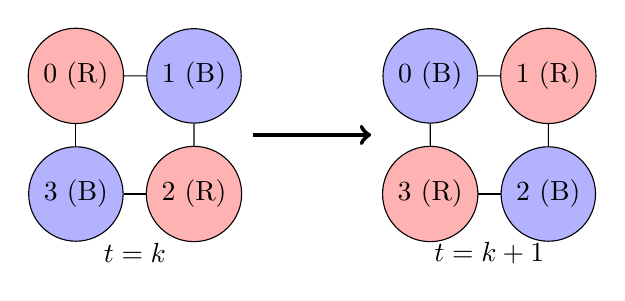
\begin{tikzpicture}[scale=1.5, auto, swap]
        % t=0
        \node[draw, circle, fill=red!30, minimum size=1cm] (0) at (0,1) {0 (R)};
        \node[draw, circle, fill=blue!30, minimum size=1cm] (1) at (1,1) {1 (B)};
        \node[draw, circle, fill=red!30, minimum size=1cm] (2) at (1,0) {2 (R)};
        \node[draw, circle, fill=blue!30, minimum size=1cm] (3) at (0,0) {3 (B)};
        \draw (0) -- (1);
        \draw (1) -- (2);
        \draw (2) -- (3);
        \draw (3) -- (0);
        \node at (0.5, -0.5) {$t=k$};

        \draw[->, ultra thick] (1.5, 0.5) -- (2.5, 0.5);

        % t=1
        \node[draw, circle, fill=blue!30, minimum size=1cm] (0b) at (3,1) {0 (B)};
        \node[draw, circle, fill=red!30, minimum size=1cm] (1b) at (4,1) {1 (R)};
        \node[draw, circle, fill=blue!30, minimum size=1cm] (2b) at (4,0) {2 (B)};
        \node[draw, circle, fill=red!30, minimum size=1cm] (3b) at (3,0) {3 (R)};
        \draw (0b) -- (1b);
        \draw (1b) -- (2b);
        \draw (2b) -- (3b);
        \draw (3b) -- (0b);
        \node at (3.5, -0.5) {$t=k+1$};

    \end{tikzpicture}
    \caption{Counterexample: A square graph with alternating colors oscillates indefinitely.}
    \label{fig:counterexample}
\end{figure}

\section*{Problem 4: PageRank Warm-Up}

\subsection*{Part (a)}
Matrix $A$:
$$
P_A = \begin{pmatrix}
    2/5 & 3/10 & 3/10\\
    1/5 & 3/5 & 1/5\\
    7/10 & 1/10 & 1/5
\end{pmatrix}
$$

\textbf{1. Stationary Distribution ($\pi = \pi P_A$)}

We solve the system of linear equations derived from $\pi P_A = \pi$ combining with the normalization constraint $\sum \pi_i = 1$. Let $\pi = [\pi_1, \pi_2, \pi_3]$.

The equations are:
\begin{align*}
    (1) \quad 0.4\pi_1 + 0.2\pi_2 + 0.7\pi_3 &= \pi_1 \\
    (2) \quad 0.3\pi_1 + 0.6\pi_2 + 0.1\pi_3 &= \pi_2 \implies 0.3\pi_1 - 0.4\pi_2 + 0.1\pi_3 = 0 \\
    (3) \quad 0.3\pi_1 + 0.2\pi_2 + 0.2\pi_3 &= \pi_3 \implies 0.3\pi_1 + 0.2\pi_2 - 0.8\pi_3 = 0 \\
    (4) \quad \pi_1 + \pi_2 + \pi_3 &= 1
\end{align*}

From (2), multiply by 10: $3\pi_1 - 4\pi_2 + \pi_3 = 0 \implies \pi_3 = 4\pi_2 - 3\pi_1$.
Substitute $\pi_3$ into (3):
$3\pi_1 + 2\pi_2 - 8(4\pi_2 - 3\pi_1) = 0$
$3\pi_1 + 2\pi_2 - 32\pi_2 + 24\pi_1 = 0$
$27\pi_1 - 30\pi_2 = 0 \implies 27\pi_1 = 30\pi_2 \implies \pi_2 = 0.9\pi_1$.

Then $\pi_3 = 4(0.9\pi_1) - 3\pi_1 = 3.6\pi_1 - 3\pi_1 = 0.6\pi_1$.

Substitute into (4):
$\pi_1 + 0.9\pi_1 + 0.6\pi_1 = 1$
$2.5\pi_1 = 1 \implies \pi_1 = 0.4$.

Then $\pi_2 = 0.9(0.4) = 0.36$ and $\pi_3 = 0.6(0.4) = 0.24$.

$$ \pi_A = [0.4, 0.36, 0.24] $$

\textbf{2. Convergence Analysis}

To analyze the convergence of $\pi_0 P_A^n$, we inspect the eigenvalues of $P_A$.
The eigenvalues are $\lambda_1 = 1$, $\lambda_2 \approx 0.345$, and $\lambda_3 \approx -0.145$.

We can write the initial distribution $\pi_0$ as a linear combination of the eigenvectors $v_1, v_2, v_3$:
$$ \pi_0 = c_1 v_1 + c_2 v_2 + c_3 v_3 $$
Multiplying by $P_A^n$:
$$ \pi_0 P_A^n = c_1 (1)^n v_1 + c_2 (0.345)^n v_2 + c_3 (-0.145)^n v_3 $$
As $n \to \infty$, since $|\lambda_2| < 1$ and $|\lambda_3| < 1$, the terms $(0.345)^n$ and $(-0.145)^n$ vanish to 0.
Thus:
$$ \lim_{n\to\infty} \pi_0 P_A^n = c_1 v_1 $$
Since $v_1$ corresponds to $\lambda=1$, it is proportional to the stationary distribution $\pi_A$.
Therefore, the system \textbf{converges} to the stationary distribution.

\subsection*{Part (b)}
Matrix $B$:
$$
P_B = \begin{pmatrix}
    0 & 5/8 & 0 & 3/8\\
    1 & 0 & 0 & 0\\
    0 & 3/8 & 0 & 5/8\\
    3/4 & 0 & 1/4 & 0
\end{pmatrix} = \begin{pmatrix}
    0 & 0.625 & 0 & 0.375\\
    1 & 0 & 0 & 0\\
    0 & 0.375 & 0 & 0.625\\
    0.75 & 0 & 0.25 & 0
\end{pmatrix}
$$

\textbf{1. Stationary Distribution ($\pi = \pi P_B$)}

Equations:
\begin{align*}
    (1) \quad \pi_2 + 0.75\pi_4 &= \pi_1 \\
    (2) \quad 0.625\pi_1 + 0.375\pi_3 &= \pi_2 \\
    (3) \quad 0.25\pi_4 &= \pi_3 \implies \pi_4 = 4\pi_3 \\
    (4) \quad 0.375\pi_1 + 0.625\pi_3 &= \pi_4 \\
    (5) \quad \pi_1 + \pi_2 + \pi_3 + \pi_4 &= 1
\end{align*}

Substitute (3) into (1): $\pi_1 = \pi_2 + 3\pi_3$.
Substitute (3) into (4): $0.375\pi_1 + 0.625\pi_3 = 4\pi_3 \implies 0.375\pi_1 = 3.375\pi_3 \implies \pi_1 = 9\pi_3$.

Now find $\pi_2$ from (2): $\pi_2 = 0.625(9\pi_3) + 0.375\pi_3 = 5.625\pi_3 + 0.375\pi_3 = 6\pi_3$.

Check (1) consistency: $\pi_2 + 3\pi_3 = 6\pi_3 + 3\pi_3 = 9\pi_3 = \pi_1$. (Consistent)

Substitute all into (5):
$9\pi_3 + 6\pi_3 + \pi_3 + 4\pi_3 = 1$
$20\pi_3 = 1 \implies \pi_3 = 0.05$.

Then:
$\pi_1 = 9(0.05) = 0.45$
$\pi_2 = 6(0.05) = 0.30$
$\pi_4 = 4(0.05) = 0.20$

$$ \pi_B = [0.45, 0.30, 0.05, 0.20] $$

\textbf{2. Convergence Analysis}

The eigenvalues of $P_B$ are $\lambda_1 = 1$, $\lambda_2 = -1$, $\lambda_3 = 0.25$, and $\lambda_4 = -0.25$.
Using diagonalization, we expand $\pi_0 P_B^n$:
$$ \pi_0 P_B^n = c_1 (1)^n v_1 + c_2 (-1)^n v_2 + c_3 (0.25)^n v_3 + c_4 (-0.25)^n v_4 $$
As $n \to \infty$, terms with $\lambda_3$ and $\lambda_4$ vanish. However, the term with $\lambda_2 = -1$ oscillates between $c_2 v_2$ and $-c_2 v_2$.
$$ \pi_0 P_B^n \approx c_1 v_1 + c_2 (-1)^n v_2 $$
Since $(-1)^n$ does not converge to a single value, the distribution \textbf{does not converge}. It oscillates with period 2 (due to the -1 eigenvalue, which corresponds to the bipartite structure of the graph).

\section*{Problem 5: Training to be a Farmer}

\subsection*{Part (a)}
Let $N$ be the number of original pages. The total number of pages is now $N+1$.
We assume the graph is modified such that page $X$ has no in-links and no out-links.
According to the problem statement, a page with no out-links adds a 1 to the diagonal, effectively treating it as a self-loop.

The PageRank equation for page $X$ (denoted as $x$) is:
$$ x = \alpha \sum_{j \to X} \pi_j P_{ji} + \frac{1-\alpha}{N+1} $$
Since $X$ has no in-links from the old pages, and only a self-loop from itself (due to the sink handling rule):
$$ x = \alpha (x \cdot 1) + \frac{1-\alpha}{N+1} $$
$$ x (1 - \alpha) = \frac{1-\alpha}{N+1} $$
$$ x = \frac{1}{N+1} $$

The new page $X$ gets exactly the average PageRank $1/(N+1)$.
The PageRanks of the older pages $\tilde{r}_i$ will decrease slightly. Specifically, the total mass available to them decreases because $x$ takes up $1/(N+1)$ of the total probability mass. Each $\tilde{r}_i \approx r_i \frac{N}{N+1}$.

\subsection*{Part (b)}
We add a page $Y$ that links to $X$. $Y$ has no in-links and presumably no other out-links (so it links only to $X$). Total pages: $N+2$.

For $Y$: It has no in-links. It only receives the random jump mass.
$$ y = \alpha(0) + \frac{1-\alpha}{N+2} = \frac{1-\alpha}{N+2} $$

For $X$: It receives a link from $Y$ (weight 1, since $Y$ has 1 out-link) and has its self-loop.
$$ x = \alpha (x \cdot 1 + y \cdot 1) + \frac{1-\alpha}{N+2} $$
Substitute $y$:
$$ x(1-\alpha) = \alpha \left( \frac{1-\alpha}{N+2} \right) + \frac{1-\alpha}{N+2} $$
$$ x(1-\alpha) = \frac{1-\alpha}{N+2} (\alpha + 1) $$
$$ x = \frac{1+\alpha}{N+2} $$

Since $\alpha \approx 0.85$, $x \approx \frac{1.85}{N+2}$, which is nearly double the rank of an isolated page. The rank of $X$ significantly improves.

\subsection*{Part (c)}
We have three pages $X, Y, Z$. To maximize $x$, we should concentrate all available rank into $X$.
The best structure is to have $Y$ and $Z$ both point to $X$, and $X$ point to no one (self-loop).

Calculation:
$y = \frac{1-\alpha}{N+3}$ (only random jump)
$z = \frac{1-\alpha}{N+3}$ (only random jump)
$x = \alpha(x + y + z) + \frac{1-\alpha}{N+3}$
$x(1-\alpha) = \alpha(y+z) + \frac{1-\alpha}{N+3} = \alpha \left( \frac{2(1-\alpha)}{N+3} \right) + \frac{1-\alpha}{N+3}$
$x = \frac{2\alpha + 1}{N+3}$

Comparing to a chain/funnel $Z \to Y \to X$ (with self-loops/sinks):
If $Z \to Y$, then $z = \frac{1-\alpha}{N+3}$, $y = \alpha z + \frac{1-\alpha}{N+3} = \frac{1-\alpha}{N+3}(1+\alpha)$.
Then $x = \alpha(x+y) + \frac{1-\alpha}{N+3} \implies x = \frac{1 + \alpha + \alpha^2}{N+3}$.
Since $\alpha < 1$, we have $2\alpha > \alpha + \alpha^2$.

Thus, the optimal configuration is a \textbf{Star Topology}: $Y \to X$ and $Z \to X$. $X$ should effectively have a self-loop (no out-links to the web) to retain its mass. This yields $x = \frac{1+2\alpha}{N+3}$.

\newpage
\appendix
\section{Code Implementation} \label{app:code}

Below is the Python code used for training and evaluation:

\lstinputlisting[language=Python, caption={approximate\_centrality.py}]{../code/approximate_centrality.py}

\section{Code Output} \label{app:output}
Below is the execution log showing the training process and final results:
\lstinputlisting[language={}, caption={Execution Output}, basicstyle=\tiny\ttfamily]{output.log}

\section{Search Engine Code} \label{app:pagerank}
Below is the implementation of the PageRank algorithm:

\lstinputlisting[language=Python, caption={src/pagerank.py}]{../hw4-search-engine/src/pagerank.py}

\end{document}
